\documentclass{standalone}

\usepackage{tikz}
\usepackage{pgfplots}
\usepgfplotslibrary{statistics}
\usetikzlibrary{pgfplots.statistics}
\usepackage{etoolbox}

\newtoggle{label}
\togglefalse{label}

\pgfplotsset{compat=1.12}

\begin{document}
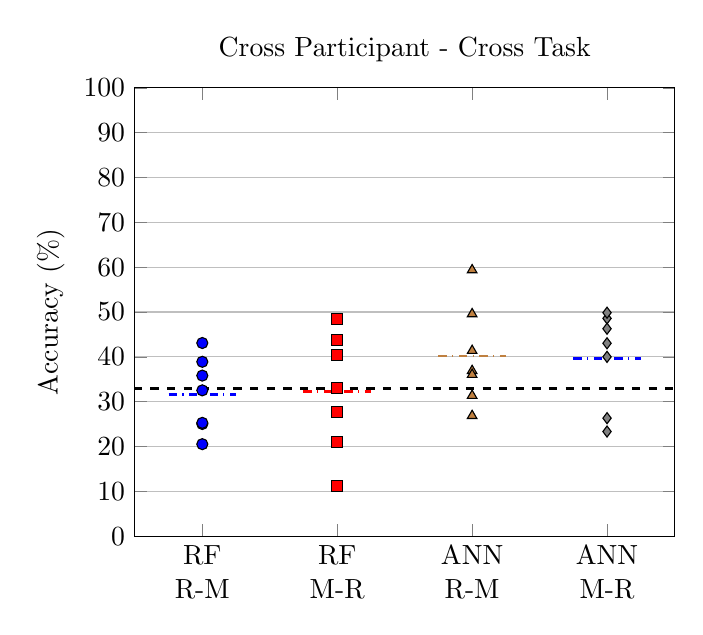
\begin{tikzpicture}
\begin{axis}[
	ymajorgrids,
	scatter/classes= {
		a={mark=*, fill=blue, draw=black},
		b={mark=square*, fill=red, draw=black},
		c={mark=triangle*, fill=brown, draw=black},
		d={mark=diamond*, fill=gray, draw=black}
	},
	ymin=0,
	ymax=100,
	xmin = .5, 
	xmax=4.5,
	ytick={0,10,...,100},
	xtick={1,2,3,4},
	xticklabel style={align=center},
	xticklabels={RF\\R-M, RF\\M-R, ANN\\R-M, ANN\\M-R},
	title=Cross Participant - Cross Task, 
	ylabel=Accuracy (\%)]

\addplot+[ mark=None, dashed, black, line width = 1pt ]
	coordinates {
	(0, 33)
	(5, 33)	
};

	% Random Forest MATB
	\addplot+[ scatter,
			only marks,
			scatter src=explicit symbolic]
	coordinates {
			(1, 25.03) [a]
			(1, 38.90) [a]
			(1, 43.09) [a]
			(1, 20.53) [a]
			(1, 35.82) [a]
			(1, 25.28) [a]
			(1, 32.53) [a]
};
\addplot+[ mark=None, dashdotted, blue, line width = 1pt ] 
	coordinates {
		(0.75, 31.59)
		(1.25, 31.59)
};

	% Random Forest RanTask
	\addplot+[ scatter,
			only marks,
			scatter src=explicit symbolic]
	coordinates {
			(2, 48.45) [b]
			(2, 11.20) [b]
			(2, 20.95) [b]
			(2, 40.39) [b]
			(2, 27.79) [b]
			(2, 43.80) [b]
			(2, 33.05) [b]
};
\addplot+[ mark=None, dashdotted, red, line width = 1pt ] 
	coordinates {
		(1.75, 32.23)
		(2.25, 32.23)
};


	% ANN MATB
	\addplot+[ scatter,
			only marks,
			scatter src=explicit symbolic]
	coordinates {
			(3, 26.86) [c]
			(3, 49.57) [c]
			(3, 36.90) [c]
			(3, 31.36) [c]
			(3, 59.37) [c]
			(3, 41.38) [c]
			(3, 36.04) [c]
};
\addplot+[ mark=None, dashdotted, brown, line width = 1pt ] 
	coordinates {
		(2.75, 40.21)
		(3.25, 40.21)
};

	% ANN RanTask
	\addplot+[ scatter,
			only marks,
			scatter src=explicit symbolic]
	coordinates {
			(4, 48.59) [d]
			(4, 26.33) [d]
			(4, 23.34) [d]
			(4, 46.28) [d]
			(4, 40.00) [d]
			(4, 49.85) [d]
			(4, 43.03) [d]
};
\addplot+[ mark=None, dashdotted, blue, line width = 1pt ] 
	coordinates {
		(3.75, 39.63)
		(4.25, 39.63)
};


\end{axis}
\end{tikzpicture}

\end{document}
















 [c]